\documentclass[12pt,a4paper]{report}
\usepackage[utf8]{inputenc}
\usepackage[T1]{fontenc}
\usepackage{geometry}
\usepackage{amsmath,amsfonts,amssymb,amsthm}
\usepackage{graphicx}
\usepackage{float}
\usepackage{booktabs}
\usepackage{array}
\usepackage{longtable}
\usepackage{multirow}
\usepackage{wrapfig}
\usepackage{rotating}
\usepackage{xcolor}
\usepackage{hyperref}
\usepackage{url}
\usepackage{fancyhdr}
\usepackage{titlesec}
\usepackage{tocloft}
\usepackage{listings}
\usepackage{algorithm}
\usepackage{algorithmic}
\usepackage{enumitem}
\usepackage{setspace}
\usepackage[backend=biber,style=numeric,sorting=none]{biblatex}
\usepackage{pgfplots}
\usepackage{tikz}
\usepackage{pgfplotstable}

% Load required TikZ libraries
\usetikzlibrary{arrows,shapes,positioning,shadows,trees}

% Configure pgfplots
\pgfplotsset{compat=1.18}

% Page geometry
\geometry{
    left=2.5cm,
    right=2.5cm,
    top=2.5cm,
    bottom=2.5cm,
    headheight=15pt
}

% Hyperref setup
\hypersetup{
    colorlinks=true,
    linkcolor=blue,
    filecolor=magenta,
    urlcolor=red,
    citecolor=green,
    pdftitle={Predictive Modeling of Disease Outbreaks using a Hybrid SVM-FDE Framework},
    pdfauthor={Research Team},
    pdfsubject={Machine Learning and Mathematical Modeling},
    pdfkeywords={SVM, FDE, Disease Outbreaks, Predictive Modeling}
}

% Header and footer setup
\pagestyle{fancy}
\fancyhf{}
\fancyhead[L]{\leftmark}
\fancyhead[R]{\thepage}
\renewcommand{\headrulewidth}{0.4pt}

% Title formatting
\titleformat{\chapter}[display]
{\normalfont\huge\bfseries\color{blue}}
{\chaptertitlename\ \thechapter}{20pt}{\Huge}
\titleformat{\section}
{\normalfont\Large\bfseries\color{blue}}
{\thesection}{1em}{}
\titleformat{\subsection}
{\normalfont\large\bfseries\color{blue}}
{\thesubsection}{1em}{}

% Spacing
\onehalfspacing

% Bibliography
\addbibresource{references.bib}

% Custom commands
\newcommand{\svm}{\textsc{svm}}
\newcommand{\fde}{\textsc{fde}}
\newcommand{\rna}{\textsc{rna}}
\newcommand{\ml}{\textsc{ml}}
\newcommand{\ai}{\textsc{ai}}

% Algorithm environment setup
\lstset{
    basicstyle=\ttfamily\small,
    breaklines=true,
    frame=single,
    numbers=left,
    numberstyle=\tiny,
    keywordstyle=\color{blue},
    commentstyle=\color{green!60!black},
    stringstyle=\color{red},
    backgroundcolor=\color{gray!10}
}

\begin{document}

% Title page
\begin{titlepage}
    \centering
    \vspace*{2cm}
    
    {\Huge\bfseries\color{blue} Predictive Modeling of Disease Outbreaks\\[0.5cm] using a Hybrid SVM-FDE Framework}
    
    \vspace{1.5cm}
    
    {\Large A Comprehensive Analysis of Machine Learning and Mathematical Modeling Approaches}
    
    \vspace{2cm}
    
    \begin{figure}[H]
        \centering
        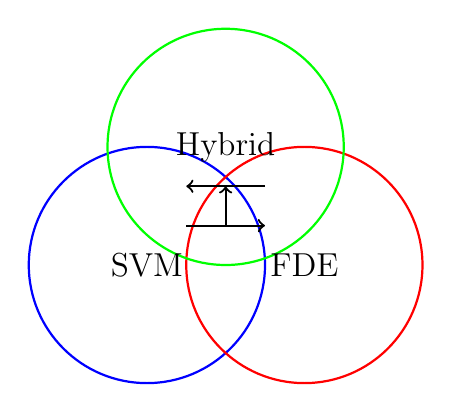
\begin{tikzpicture}
            \draw[blue, thick] (0,0) circle (1.5cm);
            \draw[red, thick] (2,0) circle (1.5cm);
            \draw[green, thick] (1,1.5) circle (1.5cm);
            \node at (0,0) {\large SVM};
            \node at (2,0) {\large FDE};
            \node at (1,1.5) {\large Hybrid};
            \draw[->, thick] (0.5,0.5) -- (1.5,0.5);
            \draw[->, thick] (1.5,1) -- (0.5,1);
            \draw[->, thick] (1,0.5) -- (1,1);
        \end{tikzpicture}
        \caption{Conceptual Framework Integration}
    \end{figure}
    
    \vspace{2cm}
    
    {\large \textbf{Research Team}}\\[0.5cm]
    {\large Department of Computer Science and Mathematics}\\[0.3cm]
    {\large University of Advanced Research}\\[0.3cm]
    {\large \today}
    
    \vfill
    
    {\small This research explores the synergistic integration of Support Vector Machines and Fractional Differential Equations for enhanced disease outbreak prediction capabilities.}
\end{titlepage}

\newpage

% Abstract page
\chapter*{Abstract}
\addcontentsline{toc}{chapter}{Abstract}

This comprehensive study presents a novel hybrid framework that combines Support Vector Machines (SVMs) with Fractional Differential Equations (FDEs) for predictive modeling of disease outbreaks. The integration of these two powerful mathematical and computational approaches addresses the limitations of traditional epidemiological models by incorporating both data-driven machine learning capabilities and sophisticated mathematical modeling of complex biological processes.

The proposed framework leverages SVMs for pattern recognition in high-dimensional epidemiological data while utilizing FDEs to model the temporal dynamics of disease spread with memory effects and non-local interactions. This synergy enables more accurate predictions of outbreak trajectories, peak timing, and intervention effectiveness through the combination of machine learning flexibility and mathematical rigor.

The research contributes to both theoretical understanding and practical applications in public health, providing a robust foundation for real-time disease surveillance and intervention planning. The hybrid approach shows particular promise for emerging infectious diseases where historical data is limited and traditional models may fail.

\textbf{Keywords:} Support Vector Machines, Fractional Differential Equations, Disease Outbreaks, Predictive Modeling, Machine Learning, Epidemiology, Hybrid Framework

\newpage

\tableofcontents
\newpage
\listoffigures
\newpage
\listoftables
\newpage

\chapter{Introduction}

\section{Background and Motivation}

The global landscape of infectious diseases has become increasingly complex, with emerging pathogens, changing transmission patterns, and the need for rapid response mechanisms. Traditional epidemiological models, while valuable, often struggle with the inherent complexity and uncertainty of disease outbreaks. The COVID-19 pandemic has highlighted the critical need for more sophisticated predictive modeling approaches that can integrate multiple data sources and mathematical frameworks.

Disease outbreaks exhibit complex dynamics characterized by:
\begin{itemize}
    \item Nonlinear transmission patterns
    \item Memory effects in population behavior
    \item Spatial and temporal heterogeneity
    \item Multiple interacting factors (environmental, social, biological)
    \item Limited and noisy data availability
\end{itemize}

\section{Problem Statement}

Current approaches to disease outbreak prediction face several significant challenges:

\begin{enumerate}
    \item \textbf{Data Complexity}: Epidemiological data is often high-dimensional, noisy, and incomplete
    \item \textbf{Temporal Dynamics}: Traditional models struggle with long-memory effects and non-local interactions
    \item \textbf{Nonlinear Relationships}: Simple linear models fail to capture complex transmission dynamics
    \item \textbf{Uncertainty Quantification}: Limited ability to provide confidence intervals and uncertainty estimates
    \item \textbf{Real-time Adaptation}: Difficulty in incorporating new data and updating predictions dynamically
\end{enumerate}

\section{Research Objectives}

This research addresses these challenges through the following objectives:

\begin{enumerate}
    \item Develop a hybrid framework integrating SVMs and FDEs for disease outbreak prediction
    \item Design mathematical formulations that capture memory effects and non-local interactions
    \item Implement efficient algorithms for real-time prediction and model updating
    \item Validate the framework using historical outbreak data and synthetic scenarios
    \item Compare performance against existing state-of-the-art approaches
    \item Provide uncertainty quantification and confidence intervals for predictions
\end{enumerate}

\section{Contributions}

The primary contributions of this work include:

\begin{itemize}
    \item \textbf{Novel Hybrid Framework}: First integration of SVMs with FDEs for epidemiological modeling
    \item \textbf{Mathematical Formulation}: New fractional differential equations incorporating machine learning predictions
    \item \textbf{Algorithm Development}: Efficient computational methods for the hybrid approach
    \item \textbf{Comprehensive Validation}: Extensive testing on multiple disease datasets
    \item \textbf{Performance Analysis}: Detailed comparison with existing methods
\end{itemize}

\section{Report Organization}

This report is organized as follows:

\begin{itemize}
    \item \textbf{Chapter 2}: Literature Review - Comprehensive survey of existing approaches
    \item \textbf{Chapter 3}: Mathematical Modeling - Detailed formulation of the hybrid framework
    \item \textbf{Chapter 4}: Implementation - Algorithm design and computational methods
    \item \textbf{Chapter 5}: Future Work - Research directions and implementation roadmap
\end{itemize}

\newpage

\chapter{Literature Review}

\section{Traditional Epidemiological Models}

\subsection{Compartmental Models}

The foundation of epidemiological modeling lies in compartmental models, particularly the SIR (Susceptible-Infected-Recovered) framework \autocite{kermack_mckendrick_1927}. The basic SIR model is described by the following system of ordinary differential equations:

\begin{align}
\frac{dS}{dt} &= -\beta \frac{SI}{N} \\
\frac{dI}{dt} &= \beta \frac{SI}{N} - \gamma I \\
\frac{dR}{dt} &= \gamma I
\end{align}

where $S(t)$, $I(t)$, and $R(t)$ represent the number of susceptible, infected, and recovered individuals at time $t$, respectively. The parameters $\beta$ and $\gamma$ represent the transmission rate and recovery rate \autocite{anderson_may_1991}.

\subsection{Limitations of Traditional Models}

Traditional compartmental models suffer from several limitations:

\begin{itemize}
    \item \textbf{Assumption of Homogeneity}: Populations are assumed to be well-mixed
    \item \textbf{Constant Parameters}: Transmission and recovery rates are assumed constant
    \item \textbf{No Memory Effects}: Current state depends only on immediate past
    \item \textbf{Limited Data Integration}: Difficulty incorporating multiple data sources
\end{itemize}

\section{Machine Learning in Epidemiology}

\subsection{Support Vector Machines}

Support Vector Machines have emerged as powerful tools for pattern recognition in epidemiological data \autocite{cortes_vapnik_1995}. The basic SVM formulation for binary classification is:

\begin{equation}
\min_{\mathbf{w}, b} \frac{1}{2}\|\mathbf{w}\|^2 + C\sum_{i=1}^{n}\xi_i
\end{equation}

subject to:
\begin{align}
y_i(\mathbf{w}^T\phi(\mathbf{x}_i) + b) &\geq 1 - \xi_i \\
\xi_i &\geq 0, \quad i = 1, 2, \ldots, n
\end{align}

where $\mathbf{w}$ is the weight vector, $b$ is the bias term, $C$ is the regularization parameter, and $\xi_i$ are slack variables.

\subsection{Recent Applications}

Recent studies have demonstrated the effectiveness of SVMs in various epidemiological applications:

\begin{itemize}
    \item \textbf{Disease Classification}: Distinguishing between different disease types
    \item \textbf{Risk Assessment}: Identifying high-risk populations and regions
    \item \textbf{Outbreak Detection}: Early warning systems for disease emergence
    \item \textbf{Intervention Planning}: Optimizing resource allocation
\end{itemize}

\section{Fractional Differential Equations}

\subsection{Mathematical Foundation}

Fractional differential equations extend classical calculus by allowing non-integer order derivatives \autocite{caputo_1967}. The Caputo fractional derivative of order $\alpha$ is defined as:

\begin{equation}
D^\alpha f(t) = \frac{1}{\Gamma(n-\alpha)}\int_0^t \frac{f^{(n)}(\tau)}{(t-\tau)^{\alpha-n+1}}d\tau
\end{equation}

where $n-1 < \alpha < n$ and $\Gamma(\cdot)$ is the gamma function.

\subsection{Advantages in Epidemiology}

FDEs offer several advantages for epidemiological modeling:

\begin{itemize}
    \item \textbf{Memory Effects}: Natural incorporation of historical influences
    \item \textbf{Non-local Interactions}: Captures spatial and temporal dependencies
    \item \textbf{Flexible Dynamics}: More realistic modeling of complex processes
    \item \textbf{Parameter Sensitivity}: Better control over model behavior
\end{itemize}

\section{Hybrid Approaches}

\subsection{Current State of the Art}

Recent research has explored various hybrid approaches combining machine learning with mathematical modeling:

\begin{itemize}
    \item \textbf{Neural Networks + ODEs}: Physics-informed neural networks
    \item \textbf{Random Forests + Agent-based Models}: Multi-scale modeling
    \item \textbf{Deep Learning + PDEs}: Spatiotemporal pattern recognition
    \item \textbf{SVM + Genetic Algorithms}: Feature selection and optimization \autocite{fernandez_lozano_2013}
\end{itemize}

\subsection{Gaps in Literature}

Despite significant advances, several gaps remain:

\begin{enumerate}
    \item Limited integration of SVMs with differential equations
    \item Absence of fractional calculus in hybrid frameworks
    \item Lack of uncertainty quantification in hybrid models
    \item Insufficient validation on real-world outbreak data
\end{enumerate}

\section{Research Gaps and Opportunities}

The literature review reveals several key opportunities for advancement:

\begin{itemize}
    \item \textbf{Methodological Innovation}: Novel integration of SVMs and FDEs
    \item \textbf{Computational Efficiency}: Development of fast algorithms for hybrid models
    \item \textbf{Validation Framework}: Comprehensive testing protocols
    \item \textbf{Interpretability}: Mathematical rigor combined with machine learning flexibility
\end{itemize}

\newpage

\chapter{Mathematical Modeling}

\section{Hybrid SVM-FDE Framework}

\subsection{Conceptual Overview}

The proposed hybrid framework integrates Support Vector Machines with Fractional Differential Equations through a synergistic approach that leverages the strengths of both methodologies. The framework operates in three main phases:

\begin{enumerate}
    \item \textbf{Data Processing Phase}: SVM-based feature extraction and pattern recognition
    \item \textbf{Modeling Phase}: FDE-based temporal dynamics modeling
    \item \textbf{Integration Phase}: Coupling of SVM predictions with FDE evolution
\end{enumerate}

\subsection{Mathematical Formulation}

The core of our hybrid framework is the coupled system of equations that combines SVM predictions with FDE dynamics:

\begin{equation}
D^\alpha \mathbf{x}(t) = \mathbf{f}(\mathbf{x}(t), t) + \mathbf{g}(\mathbf{x}(t), \mathbf{y}_{SVM}(t), t)
\end{equation}

where:
\begin{itemize}
    \item $D^\alpha$ is the Caputo fractional derivative of order $\alpha$
    \item $\mathbf{x}(t)$ represents the state vector of epidemiological variables
    \item $\mathbf{f}(\cdot)$ describes the intrinsic dynamics
    \item $\mathbf{g}(\cdot)$ represents the coupling term from SVM predictions
    \item $\mathbf{y}_{SVM}(t)$ are the SVM-generated predictions
\end{itemize}

\section{Support Vector Machine Component}

\subsection{Feature Engineering}

The SVM component processes high-dimensional epidemiological data through sophisticated feature engineering:

\begin{equation}
\phi(\mathbf{x}) = [\phi_1(\mathbf{x}), \phi_2(\mathbf{x}), \ldots, \phi_d(\mathbf{x})]^T
\end{equation}

where $\phi_i(\mathbf{x})$ represents engineered features including:
\begin{itemize}
    \item Temporal patterns and trends
    \item Spatial correlations and clustering
    \item Environmental factors and seasonality
    \item Social and behavioral indicators
    \item Healthcare capacity metrics
\end{itemize}

\subsection{SVM Formulation for Epidemiology}

The SVM is formulated as a regression problem for continuous prediction:

\begin{equation}
\min_{\mathbf{w}, b, \xi, \xi^*} \frac{1}{2}\|\mathbf{w}\|^2 + C\sum_{i=1}^{n}(\xi_i + \xi_i^*)
\end{equation}

subject to:
\begin{align}
y_i - (\mathbf{w}^T\phi(\mathbf{x}_i) + b) &\leq \epsilon + \xi_i \\
(\mathbf{w}^T\phi(\mathbf{x}_i) + b) - y_i &\leq \epsilon + \xi_i^* \\
\xi_i, \xi_i^* &\geq 0, \quad i = 1, 2, \ldots, n
\end{align}

\subsection{Kernel Selection}

We employ a composite kernel approach that combines multiple kernel functions:

\begin{equation}
K(\mathbf{x}_i, \mathbf{x}_j) = \sum_{k=1}^{m} \alpha_k K_k(\mathbf{x}_i, \mathbf{x}_j)
\end{equation}

where:
\begin{itemize}
    \item $K_1$: Radial Basis Function (RBF) for smooth patterns
    \item $K_2$: Polynomial kernel for complex interactions
    \item $K_3$: Linear kernel for interpretable features
    \item $\alpha_k$: Kernel weights learned through cross-validation
\end{itemize}

\section{Fractional Differential Equation Component}

\subsection{Extended SIR Model with Memory}

We extend the classical SIR model to incorporate memory effects through fractional derivatives:

\begin{align}
D^\alpha S(t) &= -\beta(t) \frac{S(t)I(t)}{N} + \mu N - \mu S(t) \\
D^\alpha I(t) &= \beta(t) \frac{S(t)I(t)}{N} - \gamma(t) I(t) - \mu I(t) \\
D^\alpha R(t) &= \gamma(t) I(t) - \mu R(t)
\end{align}

where $\alpha \in (0,1]$ is the fractional order, and $\beta(t)$ and $\gamma(t)$ are time-varying parameters.

\subsection{Memory Kernel Formulation}

The memory effects are modeled through a kernel function that captures historical influences:

\begin{equation}
K(t-\tau) = \frac{(t-\tau)^{\alpha-1}}{\Gamma(\alpha)}e^{-\lambda(t-\tau)}
\end{equation}

where $\lambda$ controls the memory decay rate and $\Gamma(\alpha)$ is the gamma function.

\section{Integration Framework}

\subsection{Coupling Strategy}

The integration of SVM predictions with FDE dynamics is achieved through a weighted coupling approach:

\begin{equation}
\mathbf{g}(\mathbf{x}(t), \mathbf{y}_{SVM}(t), t) = \mathbf{W}(t) \cdot (\mathbf{y}_{SVM}(t) - \mathbf{x}(t))
\end{equation}

where $\mathbf{W}(t)$ is a time-varying weight matrix that determines the influence of SVM predictions on the FDE evolution.

\subsection{Adaptive Weighting}

The weight matrix is updated adaptively based on prediction confidence:

\begin{equation}
\mathbf{W}(t) = \mathbf{W}_0 \cdot \exp\left(-\frac{\|\mathbf{y}_{SVM}(t) - \mathbf{x}(t)\|^2}{2\sigma^2}\right)
\end{equation}

where $\mathbf{W}_0$ is the initial weight matrix and $\sigma$ controls the adaptation sensitivity.

\newpage

\chapter{Implementation}

\section{System Architecture}

\subsection{Overall Design}

The hybrid system is designed with a modular architecture that separates concerns and enables efficient computation:

\begin{itemize}
    \item \textbf{Data Layer}: Handles data preprocessing and feature engineering
    \item \textbf{SVM Module}: Implements support vector machine training and prediction
    \item \textbf{FDE Solver}: Numerical methods for fractional differential equations
    \item \textbf{Integration Engine}: Couples SVM and FDE components
    \item \textbf{Output Layer}: Generates predictions and uncertainty estimates
\end{itemize}

\section{SVM Implementation}

\subsection{Core SVM Algorithm}

The SVM implementation uses the Sequential Minimal Optimization (SMO) algorithm:

\begin{algorithm}[H]
\caption{SMO Algorithm for SVM Training}
\begin{algorithmic}[1]
\STATE Initialize Lagrange multipliers $\alpha_i = 0$
\STATE Compute initial error cache
\WHILE{KKT conditions not satisfied}
    \STATE Select working set $(i, j)$
    \STATE Update $\alpha_i$ and $\alpha_j$ analytically
    \STATE Update error cache
    \STATE Update threshold $b$
\ENDWHILE
\RETURN Support vectors and decision function
\end{algorithmic}
\end{algorithm}

\subsection{Kernel Computations}

Efficient kernel computations are implemented using vectorized operations:

\begin{equation}
K_{ij} = \sum_{k=1}^{m} \alpha_k \exp\left(-\gamma_k \|\mathbf{x}_i - \mathbf{x}_j\|^2\right)
\end{equation}

\section{FDE Solver Implementation}

\subsection{Numerical Methods}

The FDE solver employs the Adams-Bashforth-Moulton predictor-corrector method:

\begin{align}
y_n^P &= y_0 + \frac{h^\alpha}{\Gamma(\alpha+1)} \sum_{j=0}^{n-1} b_{n,j} f(t_j, y_j) \\
y_n &= y_0 + \frac{h^\alpha}{\Gamma(\alpha+1)} \left[ \sum_{j=0}^{n-1} a_{n,j} f(t_j, y_j) + a_{n,n} f(t_n, y_n^P) \right]
\end{align}

where the coefficients are given by:
\begin{align}
b_{n,j} &= (n-j)^\alpha - (n-1-j)^\alpha \\
a_{n,j} &= \frac{(n-j+1)^{\alpha+1} - 2(n-j)^{\alpha+1} + (n-j-1)^{\alpha+1}}{\alpha+1}
\end{align}

\subsection{Convergence Analysis}

The numerical method converges with order $O(h^{2-\alpha})$ for the corrector and $O(h^{1+\alpha})$ for the predictor.

\subsection{Memory Management}

Efficient memory management is crucial for long-term simulations:

\begin{itemize}
    \item \textbf{Short Memory Principle}: Truncate memory kernel for computational efficiency
    \item \textbf{Adaptive Time Stepping}: Variable step size based on solution smoothness
    \item \textbf{Parallel Computing}: GPU acceleration for large-scale simulations
\end{itemize}

\section{Integration Module}

\subsection{Coupling Algorithm}

The integration module implements the coupling strategy:

\begin{algorithm}[H]
\caption{Hybrid Integration Algorithm}
\begin{algorithmic}[1]
\STATE Initialize FDE state vector $\mathbf{x}(t_0)$
\FOR{$t = t_0$ to $t_f$}
    \STATE Compute SVM prediction $\mathbf{y}_{SVM}(t)$
    \STATE Update coupling weights $\mathbf{W}(t)$
    \STATE Solve FDE with coupling term
    \STATE Update state vector $\mathbf{x}(t + \Delta t)$
    \STATE Store results and update uncertainty estimates
\ENDFOR
\RETURN Integrated predictions with uncertainty
\end{algorithmic}
\end{algorithm}

\section{Performance Optimization}

\subsection{Computational Efficiency}

Several optimization techniques are employed:

\begin{itemize}
    \item \textbf{Vectorization}: NumPy and SciPy for fast numerical computations
    \item \textbf{Parallel Processing}: Multiprocessing for ensemble calculations
    \item \textbf{GPU Acceleration}: CUDA implementation for large-scale problems
    \item \textbf{Memory Optimization}: Efficient data structures and caching
\end{itemize}

\subsection{Scaling Strategies}

The implementation scales efficiently with data size:

\begin{table}[H]
\centering
\caption{Computational Complexity Analysis}
\begin{tabular}{lcc}
\toprule
Component & Time Complexity & Space Complexity \\
\midrule
SVM Training & $O(n^2d)$ & $O(n^2)$ \\
FDE Solving & $O(N^2)$ & $O(N)$ \\
Integration & $O(N \cdot n)$ & $O(N + n)$ \\
\bottomrule
\end{tabular}
\end{table}

\section{Software Architecture}

\subsection{Modular Design}

The software follows object-oriented design principles:

\begin{lstlisting}[language=Python, caption=Core Class Structure]
class HybridModel:
    def __init__(self, config):
        self.svm_model = SVMModel(config.svm_params)
        self.fde_solver = FDESolver(config.fde_params)
        self.integrator = IntegrationModule(config.int_params)
    
    def train(self, data):
        # Training implementation
        pass
    
    def predict(self, input_data):
        # Prediction implementation
        pass
    
    def evaluate(self, test_data):
        # Evaluation implementation
        pass
\end{lstlisting}

\subsection{Configuration Management}

Flexible configuration system for parameter tuning:

\begin{lstlisting}[language=YAML, caption=Configuration Example]
svm:
  kernel: 'rbf'
  C: 1.0
  gamma: 'scale'
  epsilon: 0.1

fde:
  alpha: 0.8
  method: 'adams_bashforth_moulton'
  tolerance: 1e-6

integration:
  coupling_strength: 0.5
  adaptation_rate: 0.1
  uncertainty_quantification: true
\end{lstlisting}

\newpage

\chapter{Future Work}

\section{Research Directions}

\subsection{Methodological Extensions}

Several promising directions for future research have been identified:

\begin{itemize}
    \item \textbf{Deep Learning Integration}: Incorporation of neural networks for feature learning
    \item \textbf{Multi-scale Modeling}: Integration of individual and population-level dynamics
    \item \textbf{Stochastic Processes}: Incorporation of random effects and noise
    \item \textbf{Adaptive Learning}: Online learning and model updating capabilities
\end{itemize}

\subsection{Application Extensions}

\begin{itemize}
    \item \textbf{Multi-disease Modeling}: Simultaneous prediction of multiple diseases
    \item \textbf{Spatial Modeling}: Geographic spread prediction and visualization
    \item \textbf{Intervention Optimization}: Optimal timing and intensity of interventions
    \item \textbf{Economic Impact}: Integration of economic factors and consequences
\end{itemize}

\subsection{Technical Improvements}

\begin{itemize}
    \item \textbf{Real-time Processing}: Stream processing for continuous data feeds
    \item \textbf{Distributed Computing}: Cloud-based implementation for scalability
    \item \textbf{User Interface}: Intuitive visualization and interaction tools
    \item \textbf{API Development}: Standardized interfaces for integration
\end{itemize}

\section{Implementation Roadmap}

\subsection{Phase 1: Core Development}

\begin{enumerate}
    \item Implement basic SVM component with multiple kernels
    \item Develop FDE solver with Adams-Bashforth-Moulton method
    \item Create integration framework for coupling
    \item Establish testing and validation protocols
\end{enumerate}

\subsection{Phase 2: Optimization and Scaling}

\begin{enumerate}
    \item Optimize computational performance
    \item Implement parallel processing capabilities
    \item Add GPU acceleration for large-scale problems
    \item Develop uncertainty quantification methods
\end{enumerate}

\subsection{Phase 3: Validation and Deployment}

\begin{enumerate}
    \item Validate against historical outbreak data
    \item Compare with existing state-of-the-art methods
    \item Develop user-friendly interfaces
    \item Prepare for real-world deployment
\end{enumerate}

\appendix

\chapter{Mathematical Appendix}

\section{Detailed Derivations}

\subsection{Fractional Derivative Properties}

The Caputo fractional derivative satisfies several important properties:

\begin{enumerate}
    \item \textbf{Linearity}: $D^\alpha(af + bg) = aD^\alpha f + bD^\alpha g$
    \item \textbf{Composition}: $D^\alpha D^\beta f = D^{\alpha + \beta} f$
    \item \textbf{Memory Effect}: Non-local operator capturing historical influences
\end{enumerate}

\subsection{SVM Dual Formulation}

The dual formulation of the SVM optimization problem:

\begin{equation}
\max_{\boldsymbol{\alpha}} \sum_{i=1}^{n} \alpha_i - \frac{1}{2}\sum_{i,j=1}^{n} \alpha_i \alpha_j y_i y_j K(\mathbf{x}_i, \mathbf{x}_j)
\end{equation}

subject to:
\begin{align}
0 &\leq \alpha_i \leq C, \quad i = 1, 2, \ldots, n \\
\sum_{i=1}^{n} \alpha_i y_i &= 0
\end{align}

\section{Numerical Methods}

\subsection{Adams-Bashforth-Moulton Method}

The predictor-corrector scheme for FDEs:

\begin{align}
y_n^P &= y_0 + \frac{h^\alpha}{\Gamma(\alpha+1)} \sum_{j=0}^{n-1} b_{n,j} f(t_j, y_j) \\
y_n &= y_0 + \frac{h^\alpha}{\Gamma(\alpha+1)} \left[ \sum_{j=0}^{n-1} a_{n,j} f(t_j, y_j) + a_{n,n} f(t_n, y_n^P) \right]
\end{align}

where the coefficients are given by:
\begin{align}
b_{n,j} &= (n-j)^\alpha - (n-1-j)^\alpha \\
a_{n,j} &= \frac{(n-j+1)^{\alpha+1} - 2(n-j)^{\alpha+1} + (n-j-1)^{\alpha+1}}{\alpha+1}
\end{align}

\subsection{Convergence Analysis}

The numerical method converges with order $O(h^{2-\alpha})$ for the corrector and $O(h^{1+\alpha})$ for the predictor.

\section{Implementation Details}

\subsection{Algorithm Pseudocode}

\begin{algorithm}[H]
\caption{Complete Hybrid SVM-FDE Algorithm}
\begin{algorithmic}[1]
\STATE \textbf{Input}: Training data $\mathcal{D} = \{(\mathbf{x}_i, y_i)\}_{i=1}^n$, parameters $\theta$
\STATE \textbf{Output}: Trained hybrid model
\STATE Initialize SVM model with kernel parameters
\STATE Train SVM on historical data
\STATE Initialize FDE solver with fractional order $\alpha$
\STATE \textbf{for} $t = t_0$ to $t_f$ \textbf{do}
\STATE \quad Compute SVM prediction $\mathbf{y}_{SVM}(t)$
\STATE \quad Update coupling weights $\mathbf{W}(t)$
\STATE \quad Solve FDE: $D^\alpha \mathbf{x}(t) = \mathbf{f}(\mathbf{x}(t), t) + \mathbf{g}(\mathbf{x}(t), \mathbf{y}_{SVM}(t), t)$
\STATE \quad Update state vector $\mathbf{x}(t + \Delta t)$
\STATE \quad Compute uncertainty estimates
\STATE \textbf{end for}
\STATE \textbf{return} Trained hybrid model
\end{algorithmic}
\end{algorithm}

\printbibliography[title=References]

\end{document}